% !TeX root = ../thuthesis-example.tex

\chapter{模型上下文协议(MCP)的设计与实现}
\label{chap:mcp}

模型上下文协议(Model Context Protocol, MCP)是一种标准化协议,用于规范AI应用与数据源和工具的连接与交互。MCP提供了通用的接口标准,使AI模型能够一致地访问外部资源,类似于USB-C为物理设备提供的标准连接方式。在MCP出现前,开发者需要为每个数据源或工具实现专用连接接口,这一过程既耗时又限制了应用功能的扩展。通过MCP,开发者可以更高效地为AI应用集成外部资源,从而提升应用的能力范围和实用价值\cite{mcpspec2023}。

bolt.SE的MCP模块是该协议的实际应用实现,它支持用户配置和管理外部MCP服务器,使大语言模型(LLM)能够通过标准接口访问外部工具和数据。本章将分析MCP技术特点、在LLM驱动软件开发中的作用,以及bolt.SE中MCP模块的具体实现方案。

\section{模型上下文协议对 bolt.SE 的意义}

模型上下文协议(MCP)为 AI 驱动的软件工程带来了多方面的关键优势。首先,MCP 通过统一的接口规范,大幅简化了 AI 应用与外部工具的集成流程,显著降低了系统整合的复杂度。接口抽象机制实现了 AI 模型与工具的解耦,使各组件能够独立演进,并支持开发者灵活扩展系统功能。

MCP 支持多种类型的工具,能够覆盖不同 AI 应用的需求。例如,信息检索工具允许访问网络搜索、文档查询和数据库等外部数据源;计算工具提供数学运算、统计分析等能力,弥补 LLM 在精确计算方面的不足;文件操作工具支持文件的读写、创建和删除,是代码生成与文档处理的基础;API 调用工具封装了第三方服务接口,如天气、地图和社交媒体 API 等;系统交互工具提供命令执行与进程管理能力,而领域专用工具则面向代码分析、图形处理和自然语言处理等特定场景。

在传输层面,MCP 兼容多种协议(如 stdio、HTTP SSE 等),便于在不同部署环境下灵活应用。安全性方面,MCP 明确界定了权限边界,确保 AI 模型仅能通过受控接口访问外部资源,从而有效管控系统安全风险。

针对 LLM 驱动的软件开发,MCP 具有不可替代的价值。一方面,MCP 使 LLM 能够实时访问外部数据,突破模型知识截止的局限,保持信息的时效性。另一方面,借助 MCP,LLM 可调用各类专业工具和 API,完成其自身能力范围之外的任务,如数据分析与文件处理,从而极大拓展了应用场景和能力边界。

此外,MCP 能够引导 LLM 从可靠的外部资源获取信息,减少对参数化知识的依赖,显著提升输出的准确性并降低"幻觉"风险。在复杂任务求解中,MCP 支持 LLM 与外部工具的多轮交互,实现分步骤问题求解与中间结果验证。其安全机制亦确保 LLM 能在保护隐私的前提下访问用户私有数据,实现功能性与安全性的平衡。

bolt.SE 将 MCP 深度融合于系统设计之中,通过标准化工具接口,促进 LLM 与外部工具及数据源的协同工作,使开发者能够通过自然语言交互获得工具增强的智能辅助,既保留 LLM 的灵活创造力,又引入专业工具的精确性与扩展能力。

\section{bolt.SE中的MCP功能实现}

图\ref{fig:mcp_workflow}展示了MCP在bolt.SE中的完整交互流程,涵盖了配置、连接、工具调用和结果返回四个主要阶段。首先是配置阶段,用户通过界面配置MCP服务器,系统从IndexedDB加载现有配置并显示,支持配置stdio和SSE两种传输类型服务器;其次是连接阶段,系统根据配置类型分别创建对应的客户端实例,对stdio类型服务器通过命令行参数启动本地进程并建立管道通信,对SSE类型服务器则通过HTTP请求建立事件流连接;第三是工具发现阶段,所有服务器连接成功后向客户端提供其可用工具列表,系统将这些工具信息整合并展示给用户;最后是工具调用阶段,当用户发送对话消息时,系统准备包含MCP工具的上下文传递给AI,AI可根据需要调用本地或远程工具,执行结果通过对应服务器返回,并最终整合到对话响应中展示给用户。流程最后还包括会话结束时系统关闭所有MCP连接的资源回收过程。

\begin{figure}[H]
  \centering
  \makebox[\textwidth][c]{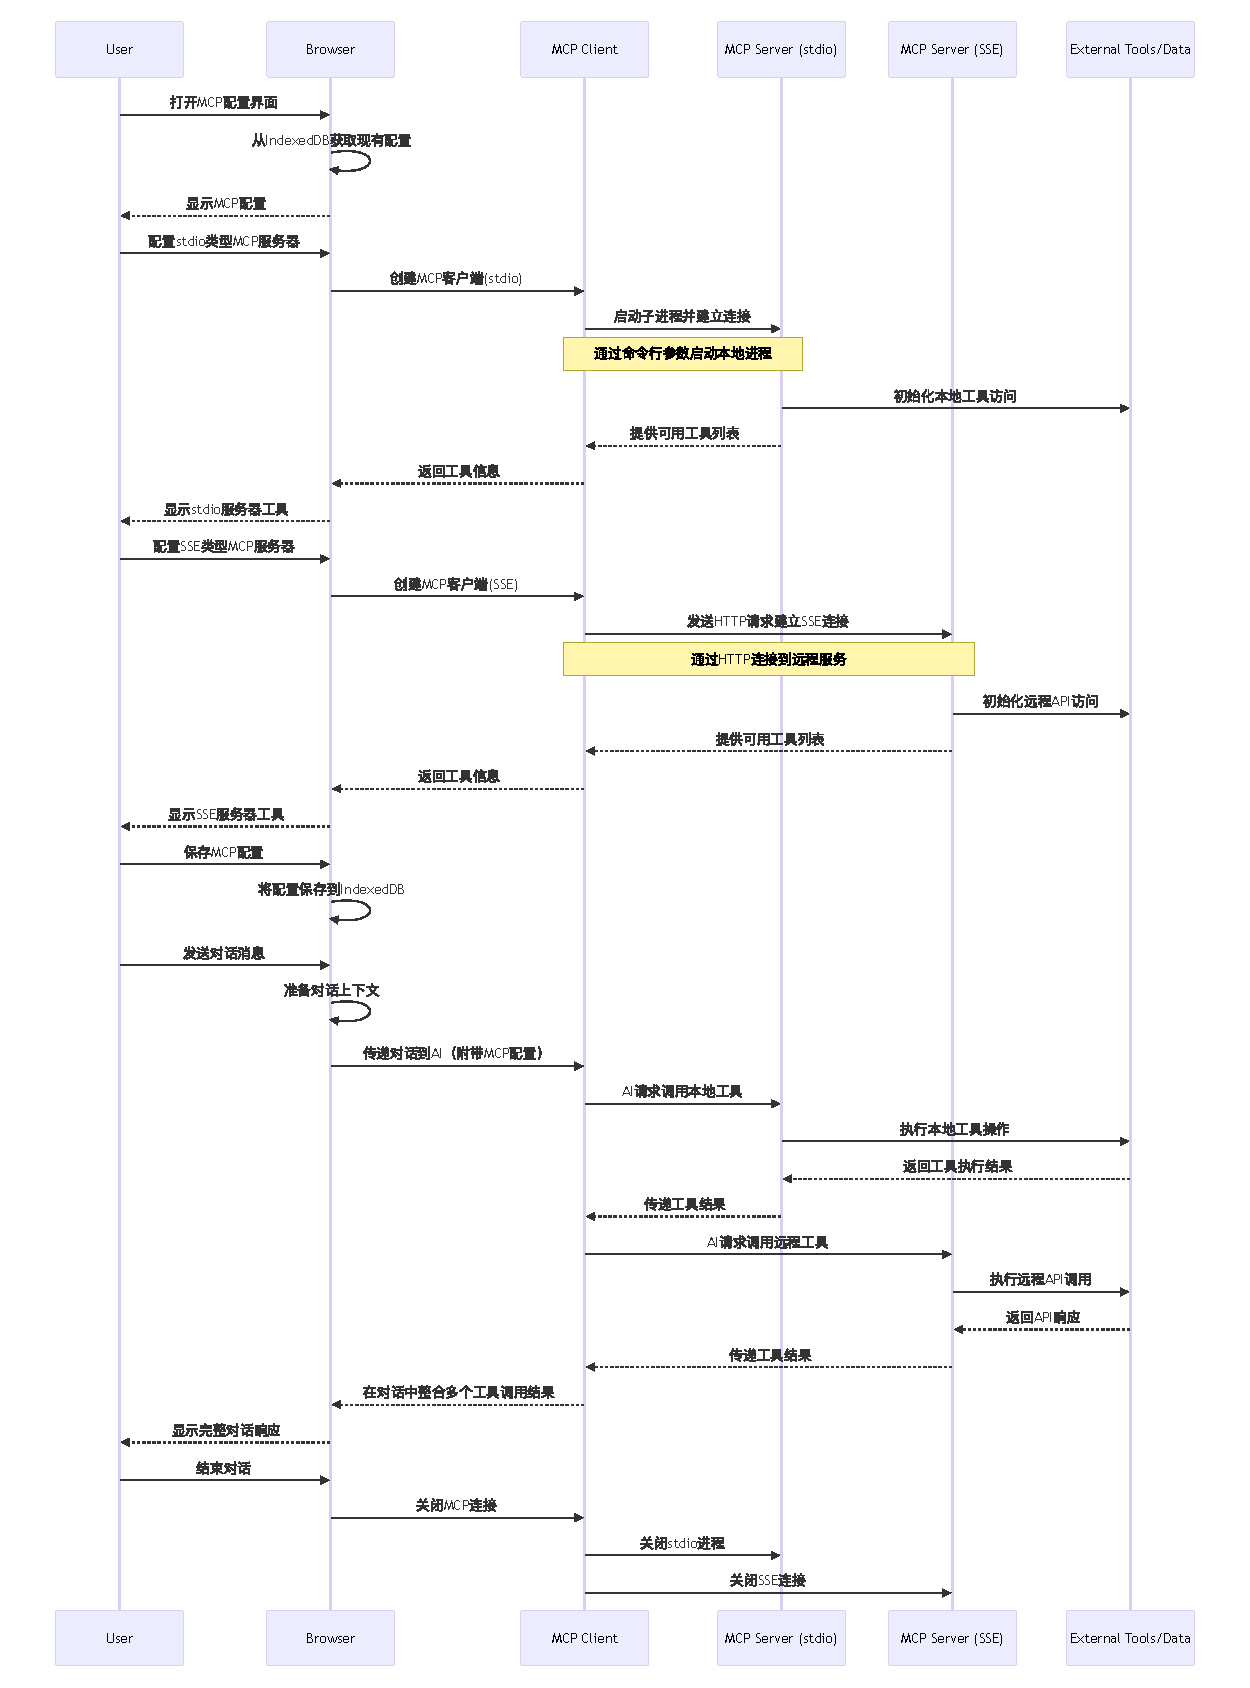
\includegraphics[width=1.1\textwidth]{figures/mcp_sequence.pdf}}
  \caption{MCP工作流程图:展示用户配置、服务器连接和工具调用的完整流程}
  \label{fig:mcp_workflow}
\end{figure}

图\ref{fig:mcp_state}展示了MCP系统的状态转换流程,刻画了从应用启动到服务关闭的各个细节状态。状态图分为四个主要区域:客户端初始化、服务器交互、对话流程和会话结束。

\begin{figure}[H]
  \centering
  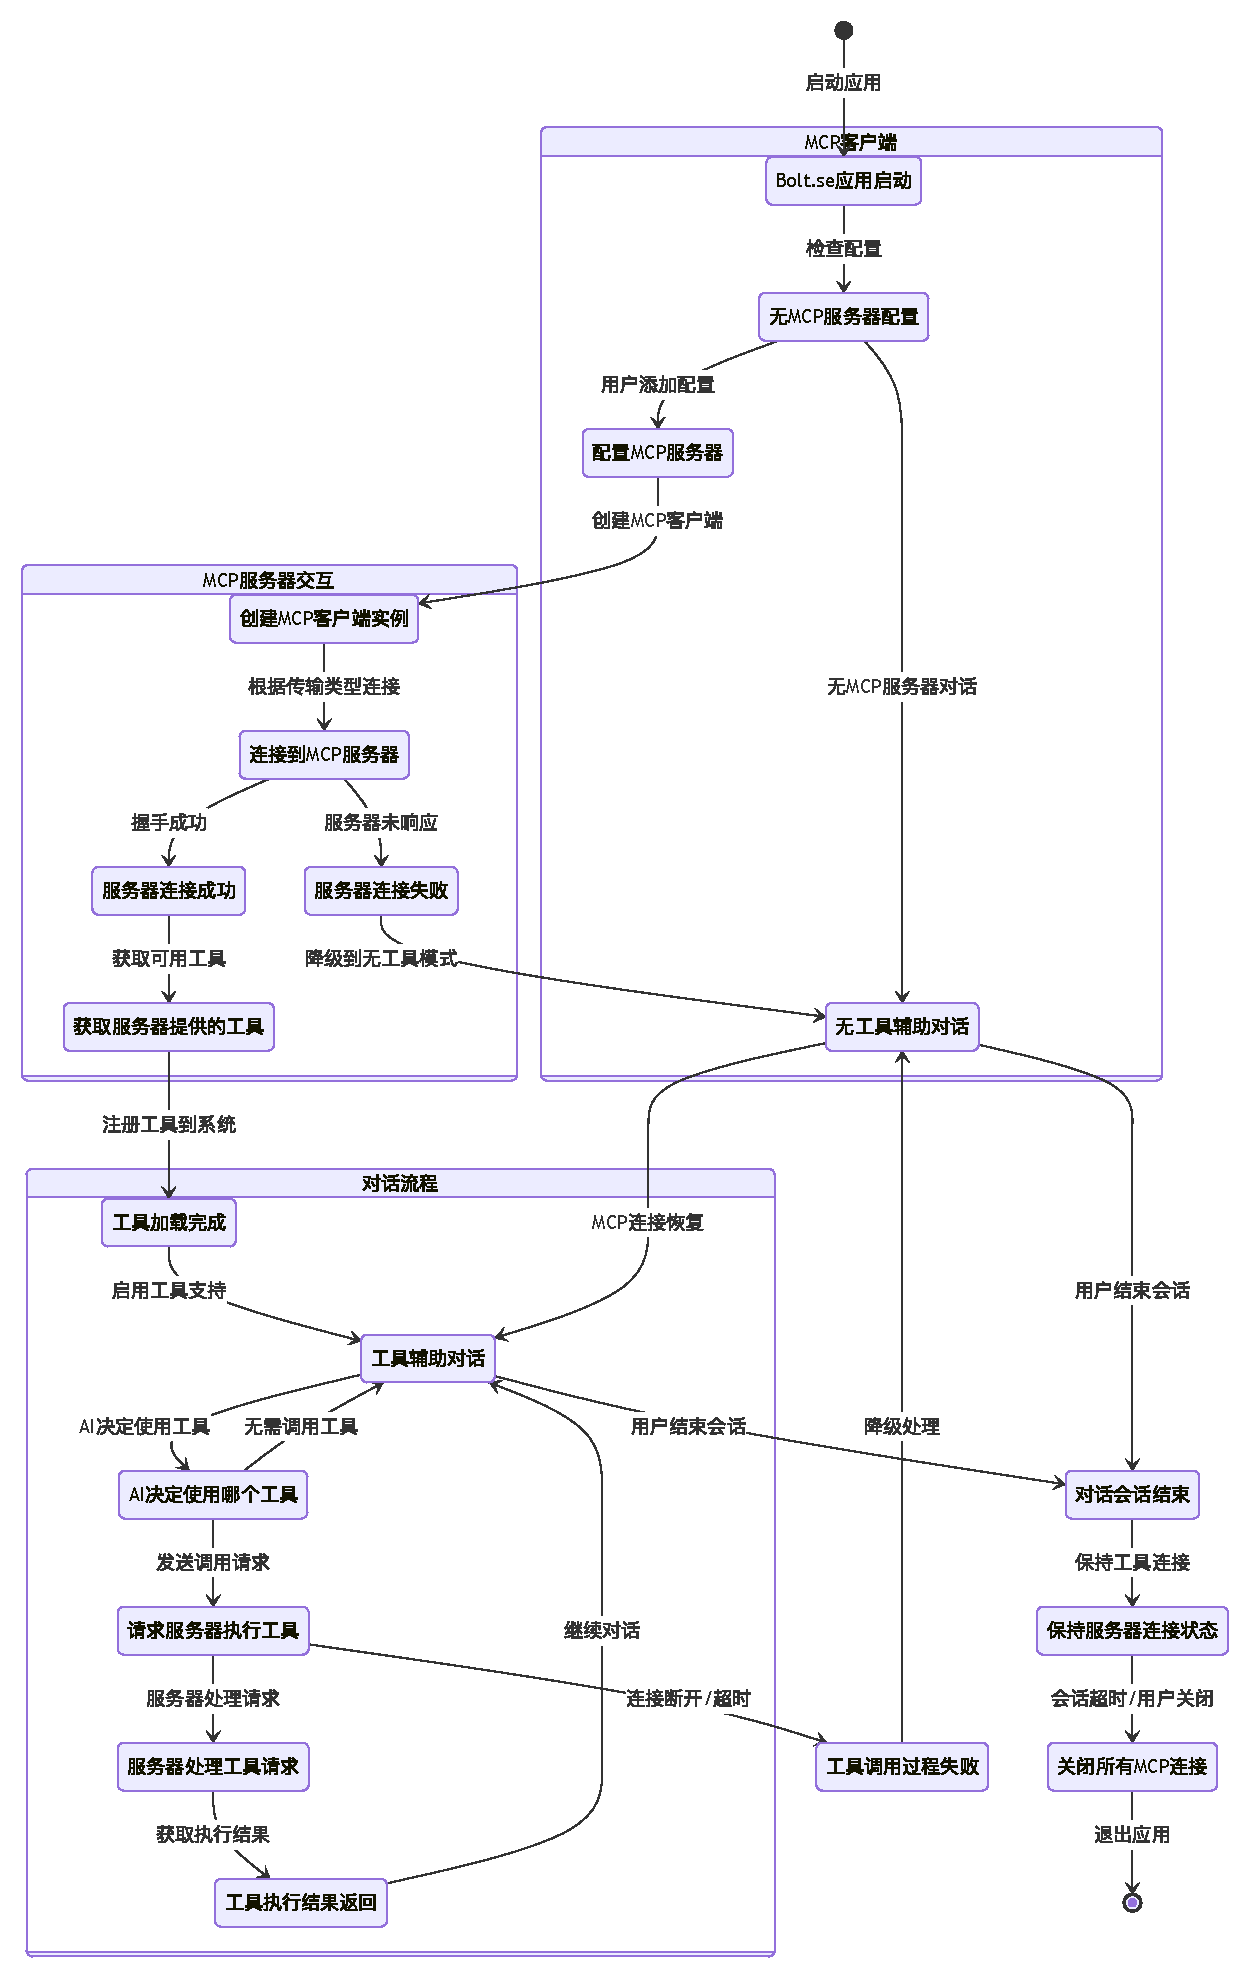
\includegraphics[width=\textwidth]{figures/mcp_state.pdf}
  \caption{MCP状态图:描述MCP连接的各状态及转换关系,从初始配置到工具调用的完整流程}
  \label{fig:mcp_state}
\end{figure}

如图\ref{fig:mcp_class}所示的类图展示了MCP功能的各组件间的关系:

\begin{figure}[H]
  \centering
  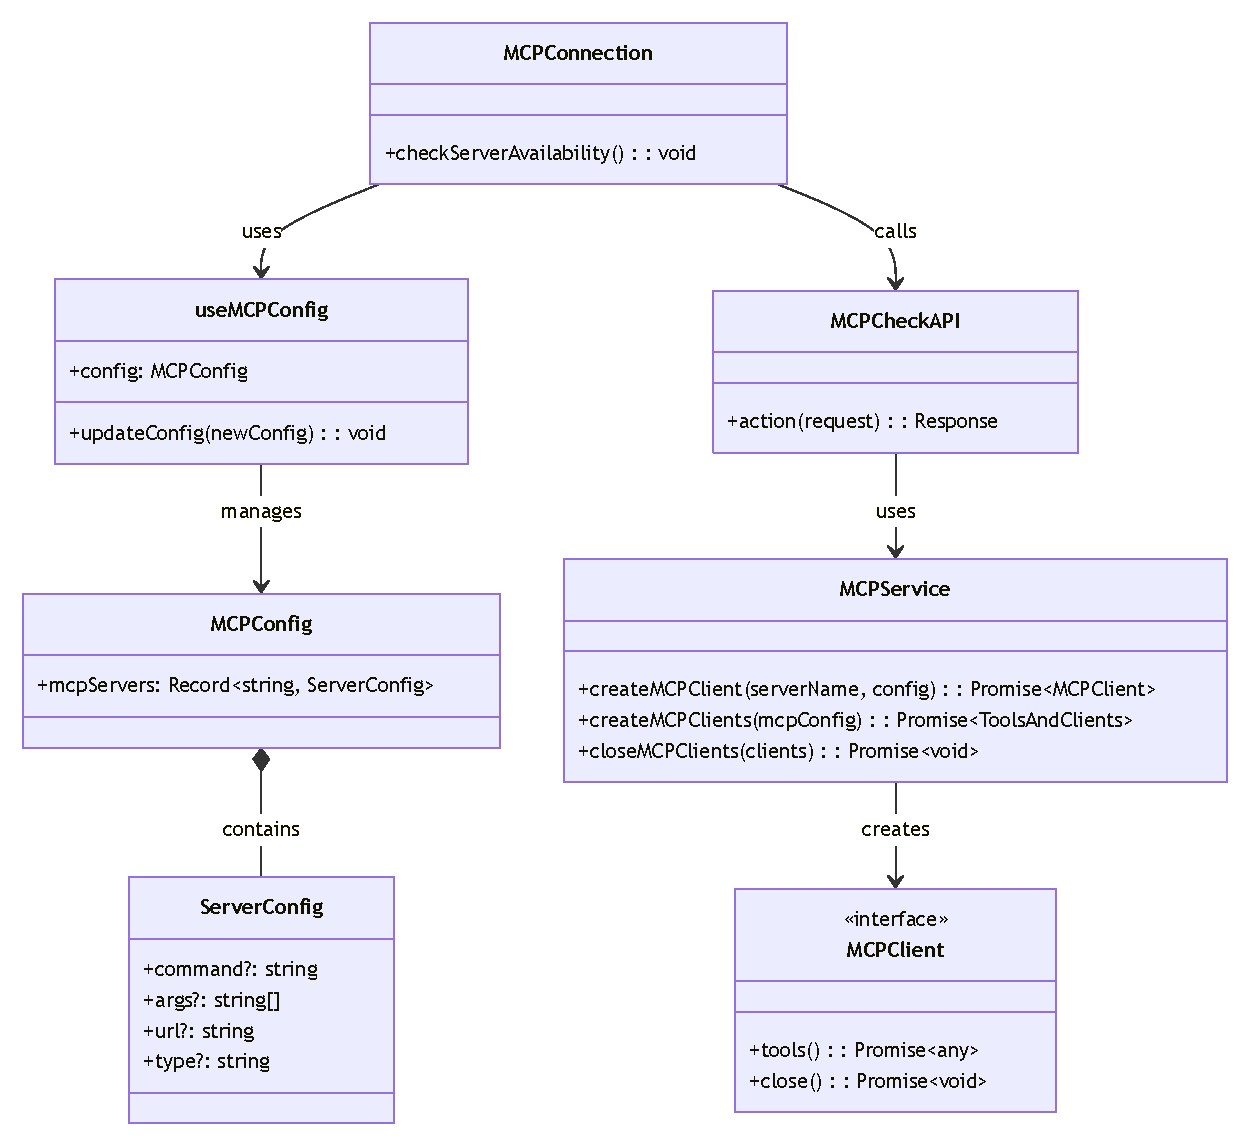
\includegraphics[width=\textwidth]{figures/mcp_class.pdf}
  \caption{MCP数据模型类图:展示系统中MCP相关模块的类结构及其关系,包括配置管理、服务创建和连接检查}
  \label{fig:mcp_class}
\end{figure}

主要组件包括:

\begin{enumerate}
  \item 配置管理组件:
    \begin{itemize}
      \item \texttt{MCPConfig}:顶层配置类,管理服务器映射表
      \item \texttt{ServerConfig}:服务器配置类,根据传输类型定义不同属性
      \item \texttt{useMCPConfig}:React Hook接口,提供配置状态管理功能
      \item \texttt{IndexedDB存储}:持久化存储机制,确保配置跨会话保存
    \end{itemize}
  
  \item 服务层组件:
    \begin{itemize}
      \item \texttt{MCPClient}:客户端接口,定义工具获取和连接管理方法
      \item \texttt{MCPService}:服务管理类,负责客户端创建与生命周期
      \item \texttt{createMCPClient}:工厂函数,根据配置创建适当类型客户端
    \end{itemize}
  
  \item 用户界面与API组件:
    \begin{itemize}
      \item \texttt{MCPConnection}:配置编辑与状态监控界面
      \item \texttt{MCPCheckAPI}:服务器可用性检查的REST端点
    \end{itemize}
  
  \item AI交互组件:
    \begin{itemize}
      \item 工具上下文注入模块:将工具描述添加到AI对话上下文
      \item 工具调用处理模块:执行工具请求并处理返回结果
    \end{itemize}
\end{enumerate}

其中,在MCP配置的设计上,bolt.SE参考Anthropic Desktop实现了的MCP配置格式,用户只需在配置界面中粘贴JSON格式的服务器定义,系统会自动检测连接性并将可用工具注册到LLM的工具选项中,无需额外设置即可在对话中使用。系统支持两种类型的MCP服务器,分别是本地进程型和远程SSE型。以下是典型配置示例:

\begin{minted}{json}
{
  "mcpServers": {
    "everything": {
      "command": "npx",
      "args": [
        "-y",
        "@modelcontextprotocol/server-everything"
      ]
    },
    "remote-sse": {
      "type": "sse",
      "url": "http://localhost:8000/sse"
    }
  }
}
\end{minted}

在这个配置中,"everything"是本地进程型服务器,通过command和args指定启动命令和参数;"remote-sse"则是远程SSE型服务器,通过type和url指定连接方式和地址。本地进程型服务器更适合访问本机资源(如文件系统、本地数据库),而SSE型服务器适合连接远程服务和API(如天气服务、企业内部服务)。

MCP服务器配置支持以下主要属性:
\begin{itemize}
  \item \texttt{command}:指定执行程序命令(如npx、node、python等)
  \item \texttt{args}:命令行参数数组,支持指定包名、路径、运行参数等
  \item \texttt{type}:传输类型(省略则默认为stdio,或明确指定为sse)
  \item \texttt{url}:SSE服务器的访问地址(仅在type为sse时使用)
  \item \texttt{env}:环境变量对象,用于传递API密钥等敏感信息
\end{itemize}

用户配置完成后,bolt.SE会自动检测并连接MCP服务器,扫描可用的工具定义,并将它们注册到对话上下文中,使LLM能够在适当的时机调用这些工具来扩展其能力。

\section{实例应用场景}
\label{sec:mcp-iotdb-demo}

本节以"MCP协同IoTDB与OpenAPI构建交互式前端应用"为例,展示MCP在实际应用中的完整流程与价值。


首先,开发环境部署IoTDB 2.0.2实例,并将名为\texttt{battery\_data}的样例数据表写入30条监测数据(包含电压、电流等参数)。系统通过两种方式暴露数据库能力:MCP通道使用\texttt{remote-sse}服务器提供三个核心工具(\textit{list\_tables}、\textit{describe\_table}和\textit{read\_query}),供LLM进行表结构分析和数据查询;同时,REST通道通过IoTDB内置的REST Service V2,将查询接口\texttt{/rest/table/v1/query}按OpenAPI 3.0规范描述。

图~\ref{fig:mcp-config}展示了bolt.SE的MCP配置界面。系统通过以下配置成功发现三个IoTDB工具:

\begin{minted}{json}
{
  "mcpServers": {
    "remote-sse": {
      "type": "sse",
      "url": "http://localhost:8000/sse"
    }
  }
}
\end{minted}

\begin{figure}[H]
  \centering
  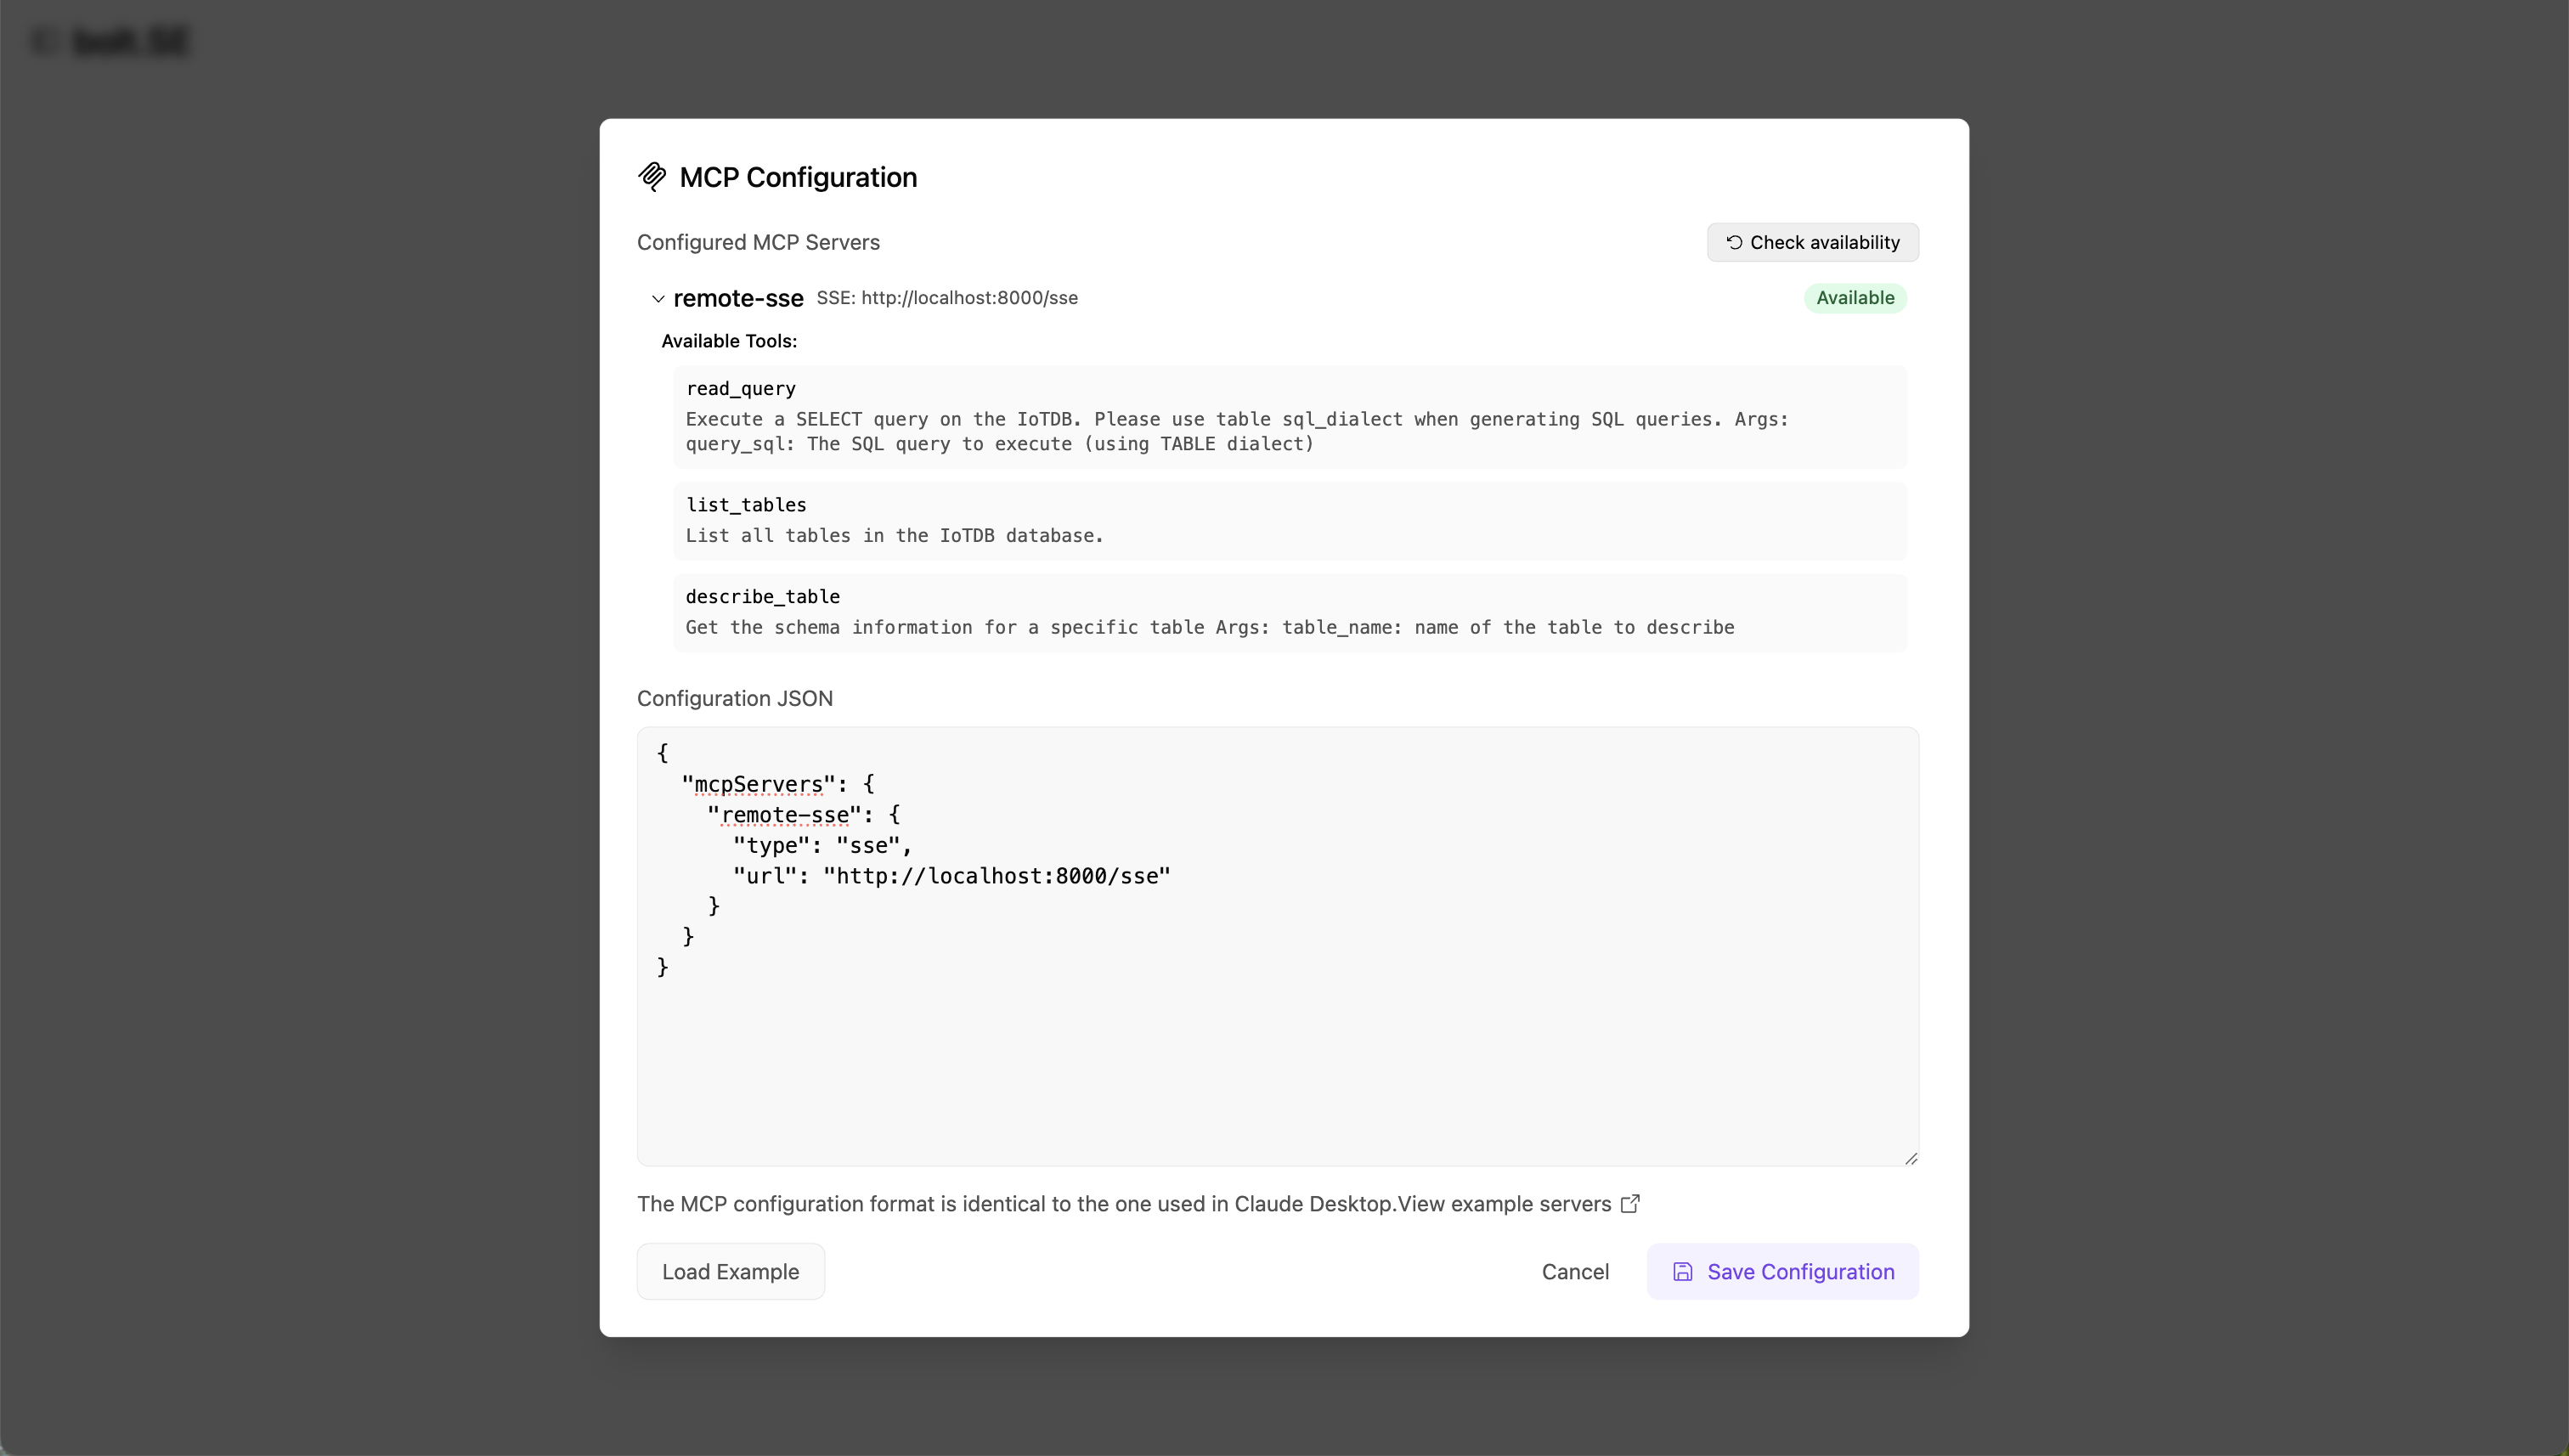
\includegraphics[width=\textwidth]{figures/screenshots/iotdb-demo/mcp-config.png}
  \caption{\texttt{remote-sse}服务器配置与IoTDB工具发现}
  \label{fig:mcp-config}
\end{figure}

同时,开发者将IoTDB查询接口按OpenAPI 3.0规范描述,并在bolt.SE的\textit{Edit actions}界面完成配置,仅保留\textit{queryTableData}动作供LLM调用。

\begin{minted}{yaml}
paths:
  /rest/table/v1/query:
    post:
      operationId: queryTableData
      summary: Execute a SQL query on the IoTDB table
      requestBody:
        required: true
        content:
          application/json:
            schema:
              type: object
              required: [database, sql]
\end{minted}

\begin{figure}[H]
  \centering
  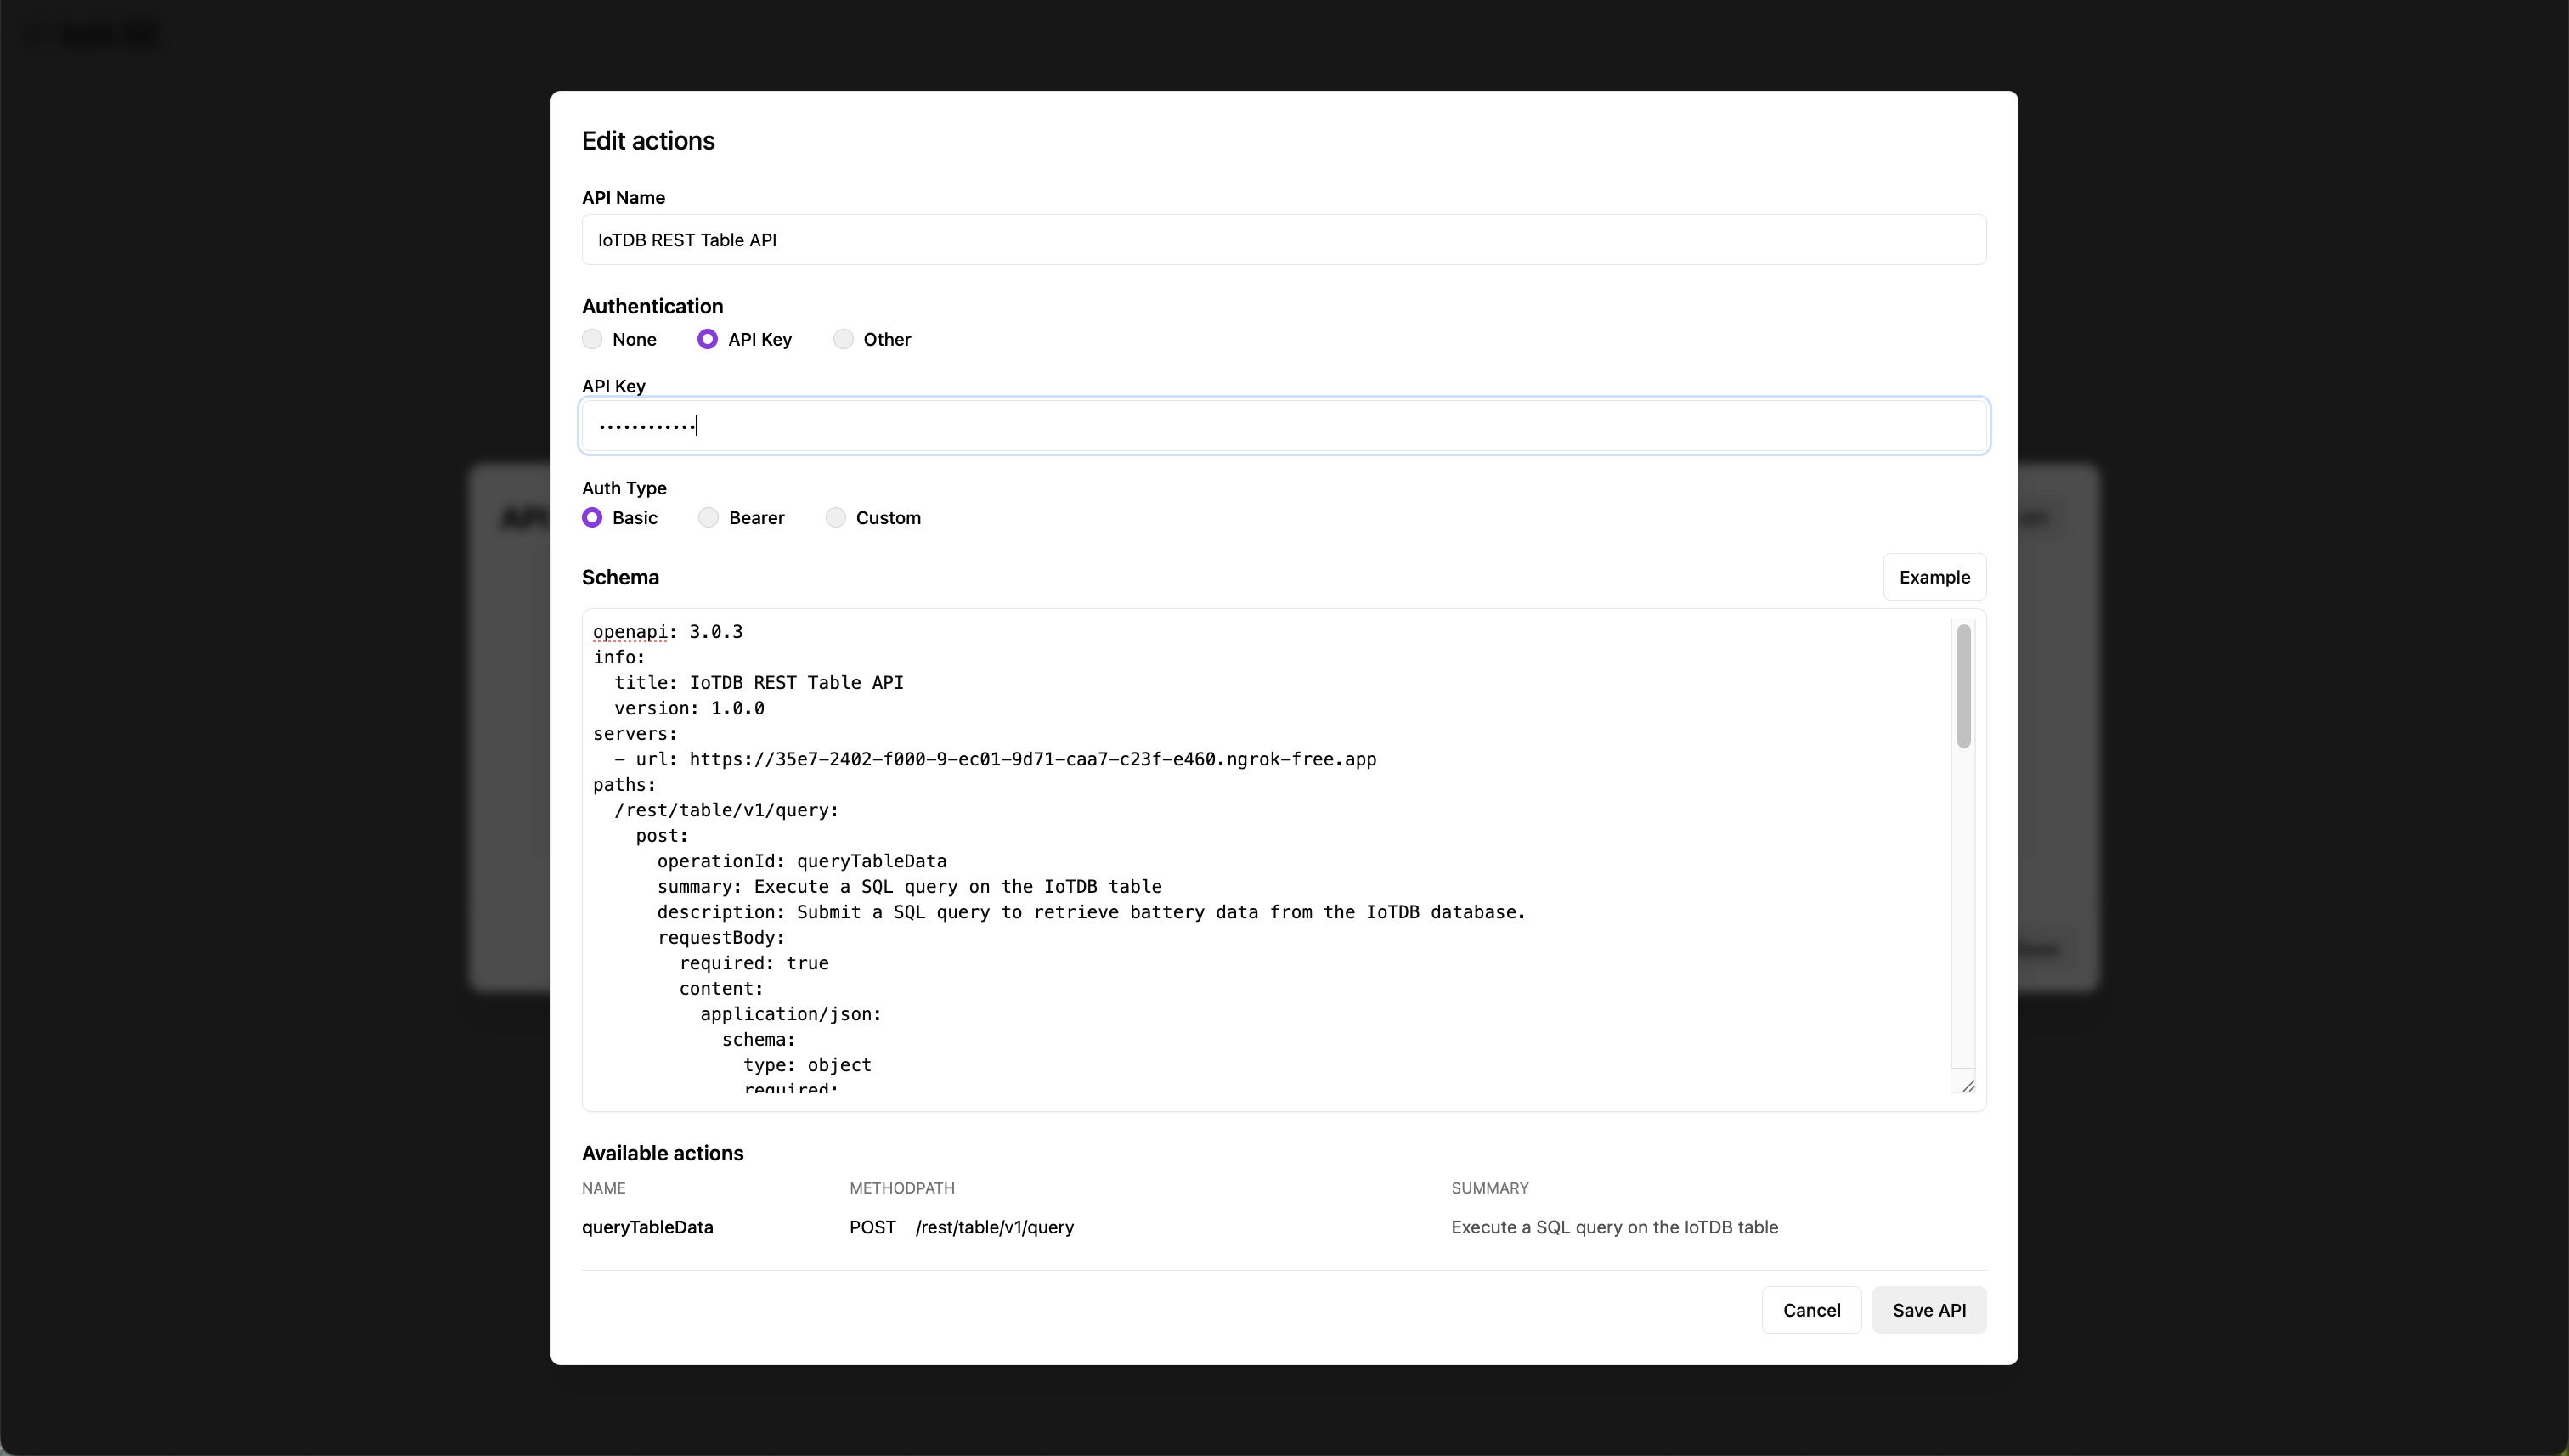
\includegraphics[width=\textwidth]{figures/screenshots/iotdb-demo/openapi-editor.png}
  \caption{OpenAPI文档编辑与认证配置界面}
  \label{fig:openapi-editor}
\end{figure}

\begin{figure}[H]
  \centering
  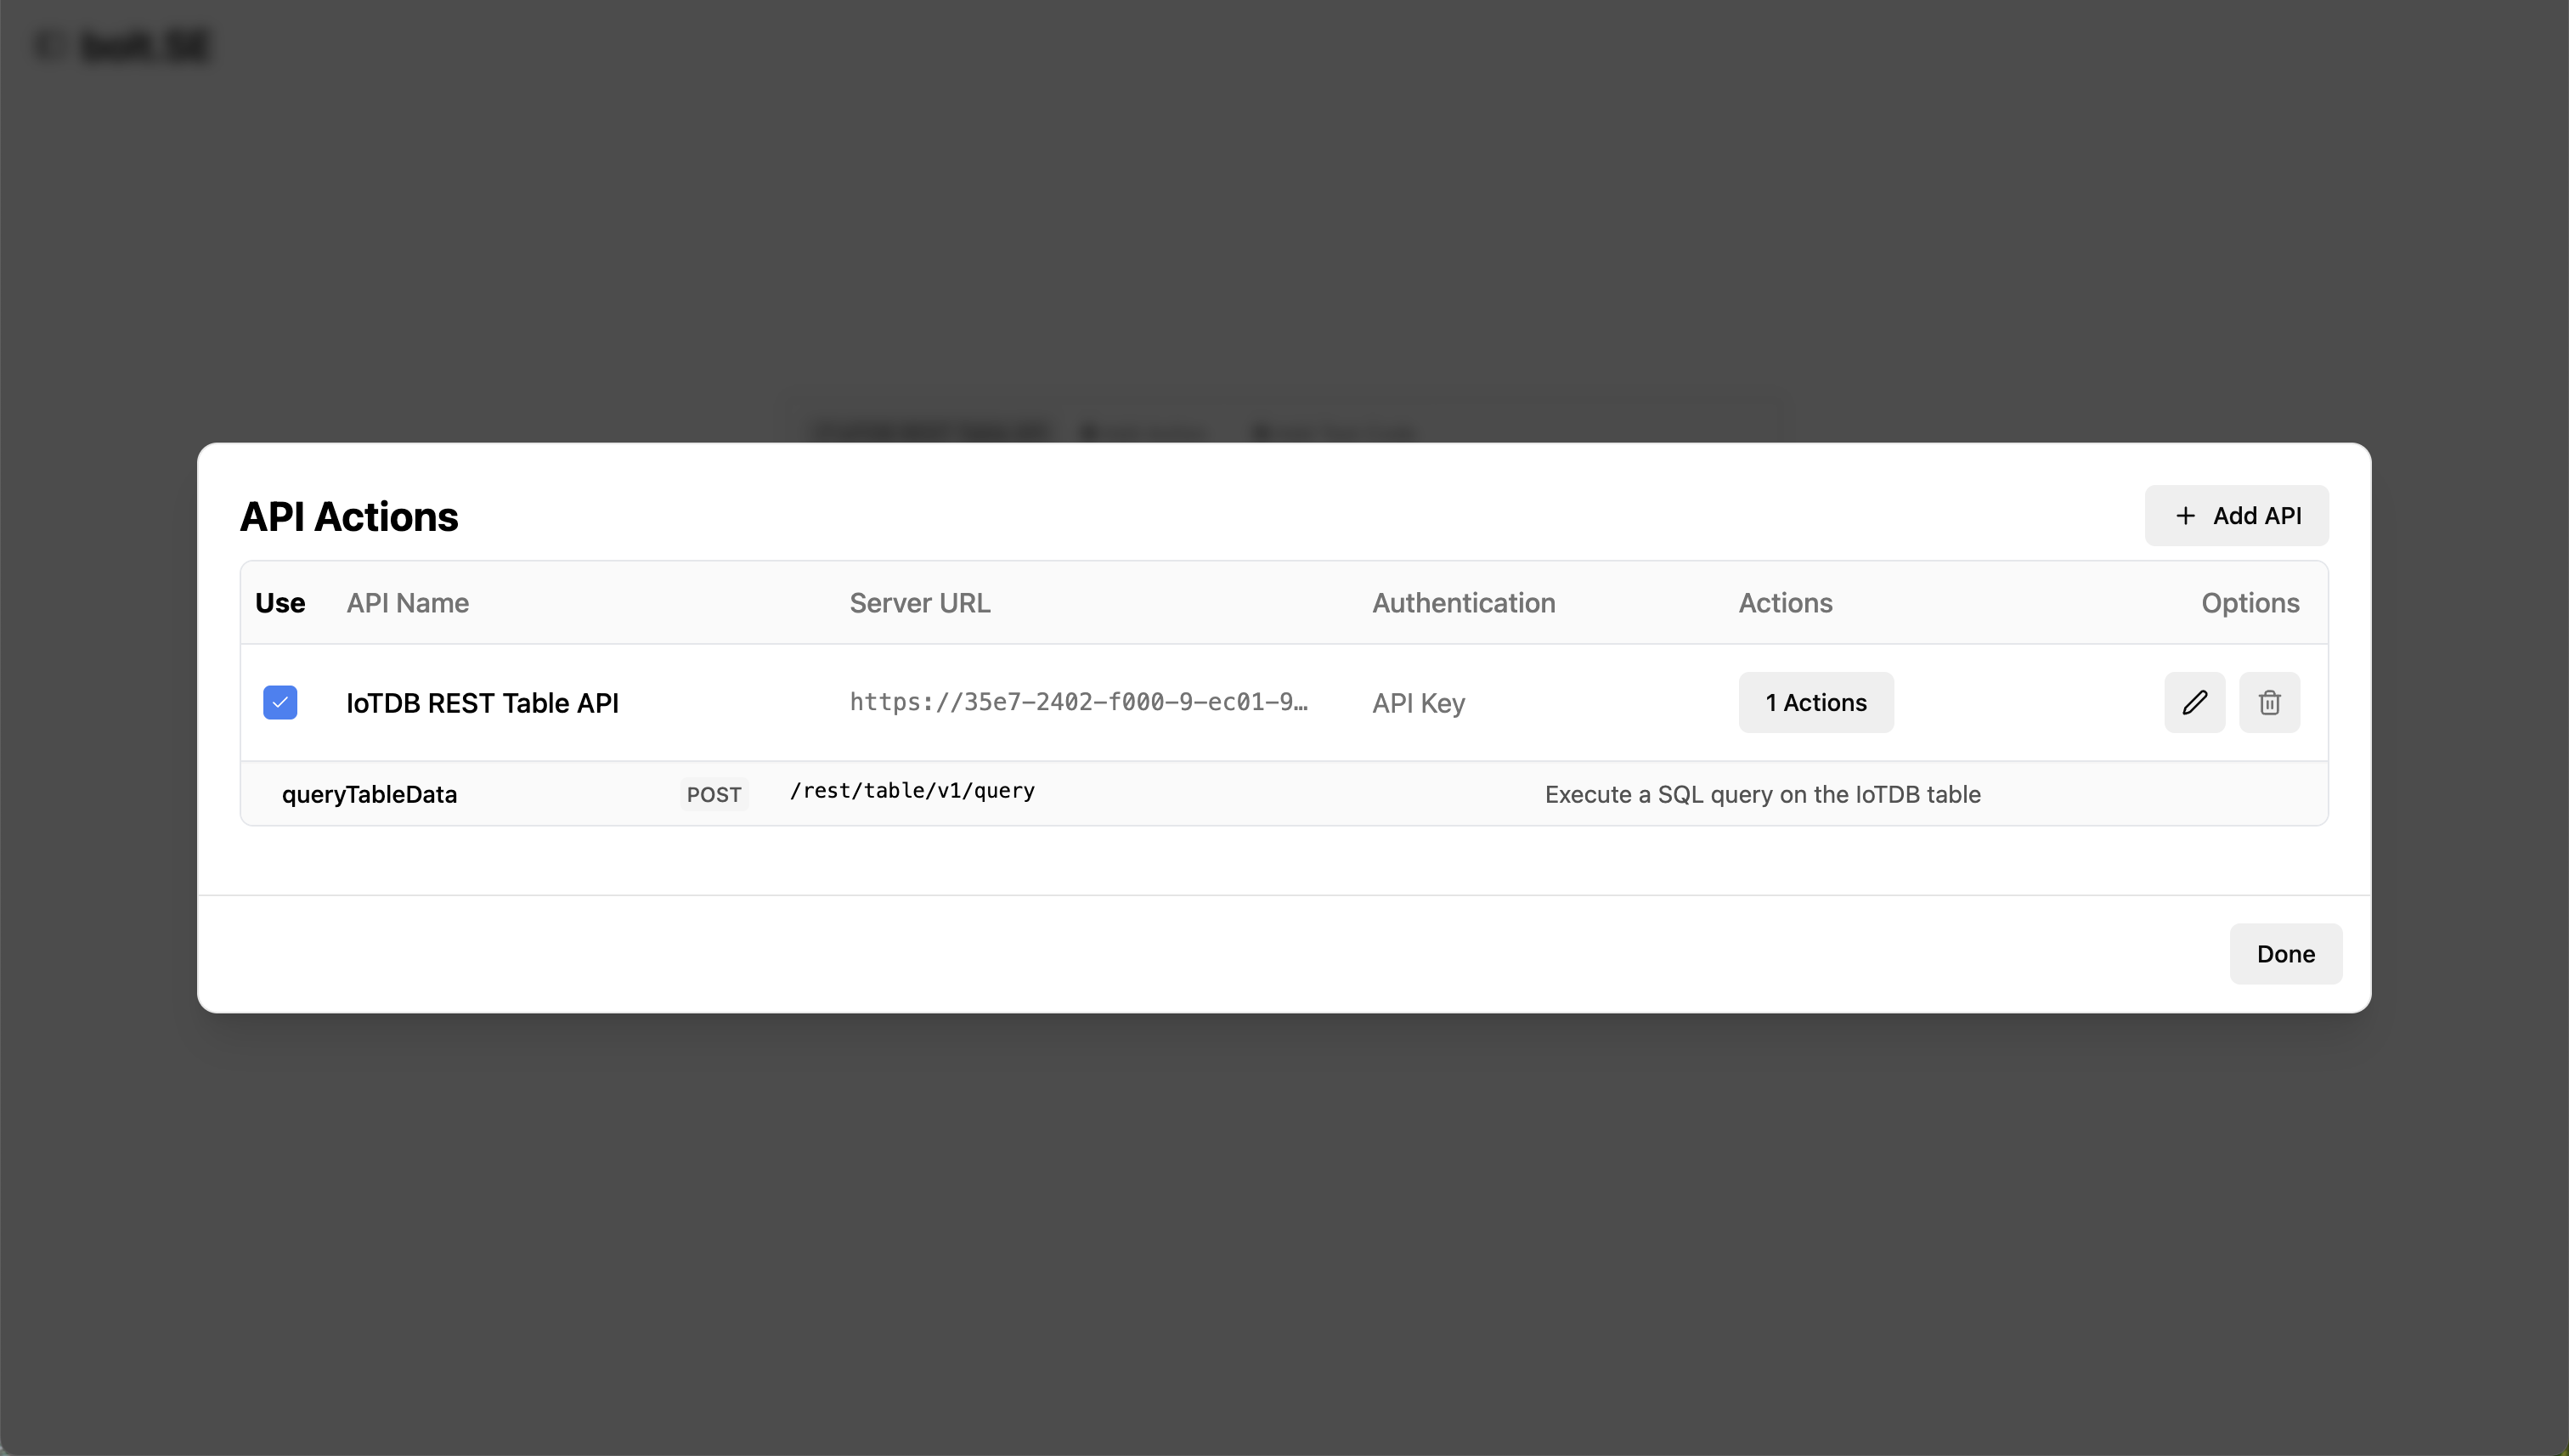
\includegraphics[width=\textwidth]{figures/screenshots/iotdb-demo/api-actions.png}
  \caption{最终配置的API动作列表}
  \label{fig:api-actions}
\end{figure}

完成配置后,开发者向系统提交以自然语言描述的提示:"Build a basic app that displays IoTDB data in a graph. Please use the tool to check the current database structure. Add a "Reload" button to refresh the data by calling the API."


系统通过以下步骤响应:

\begin{enumerate}
  \item LLM首先识别需要了解数据结构,顺序调用三个MCP工具(图~\ref{fig:mcp-call}):
    \begin{itemize}
      \item \textit{list\_tables}:确认系统中只有\texttt{battery\_data}表
      \item \textit{describe\_table}:获取表的列名及数据类型定义
      \item \textit{read\_query}:通过\verb|SELECT * FROM battery_data LIMIT 5|抽样分析数据分布
    \end{itemize}
  
  \item 随后LLM识别需要实现数据刷新功能,调用OpenAPI动作\textit{queryTableData}构建前端刷新逻辑
  
  \item 最后LLM基于获取的数据结构和API能力生成完整应用代码
\end{enumerate}

\begin{figure}[H]
  \centering
  \begin{subfigure}{0.48\textwidth}
    \centering
    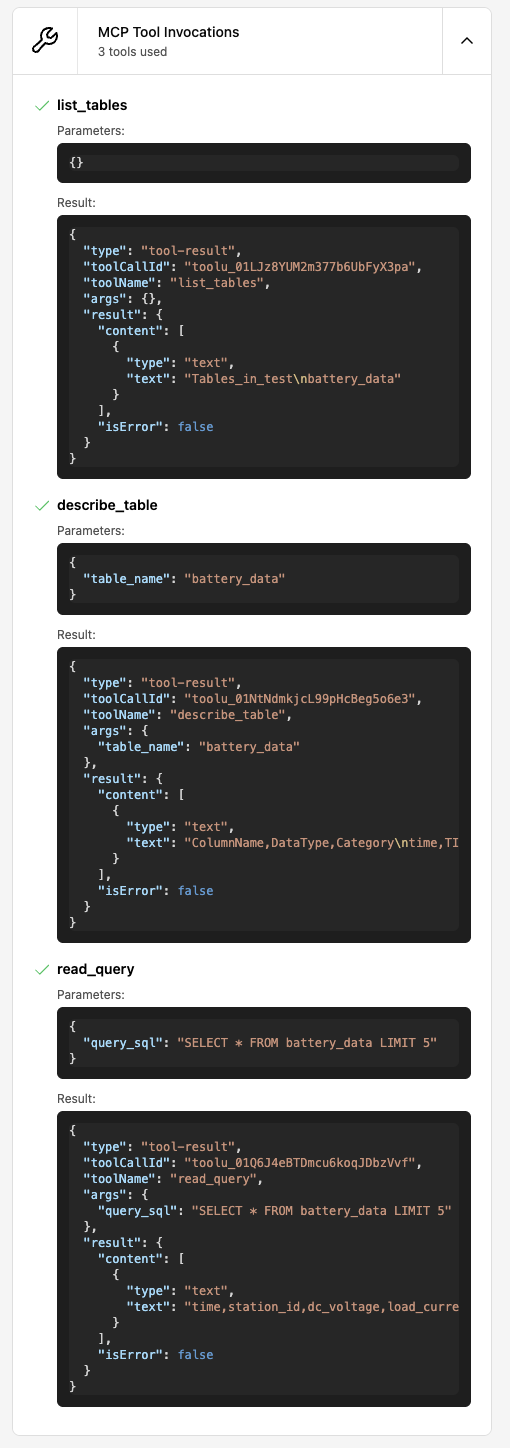
\includegraphics[width=\textwidth]{figures/screenshots/iotdb-demo/mcp-call.png}
    \caption{LLM顺序调用IoTDB相关MCP工具}
    \label{fig:mcp-call}
  \end{subfigure}
  \hfill
  \begin{subfigure}{0.48\textwidth}
    \centering
    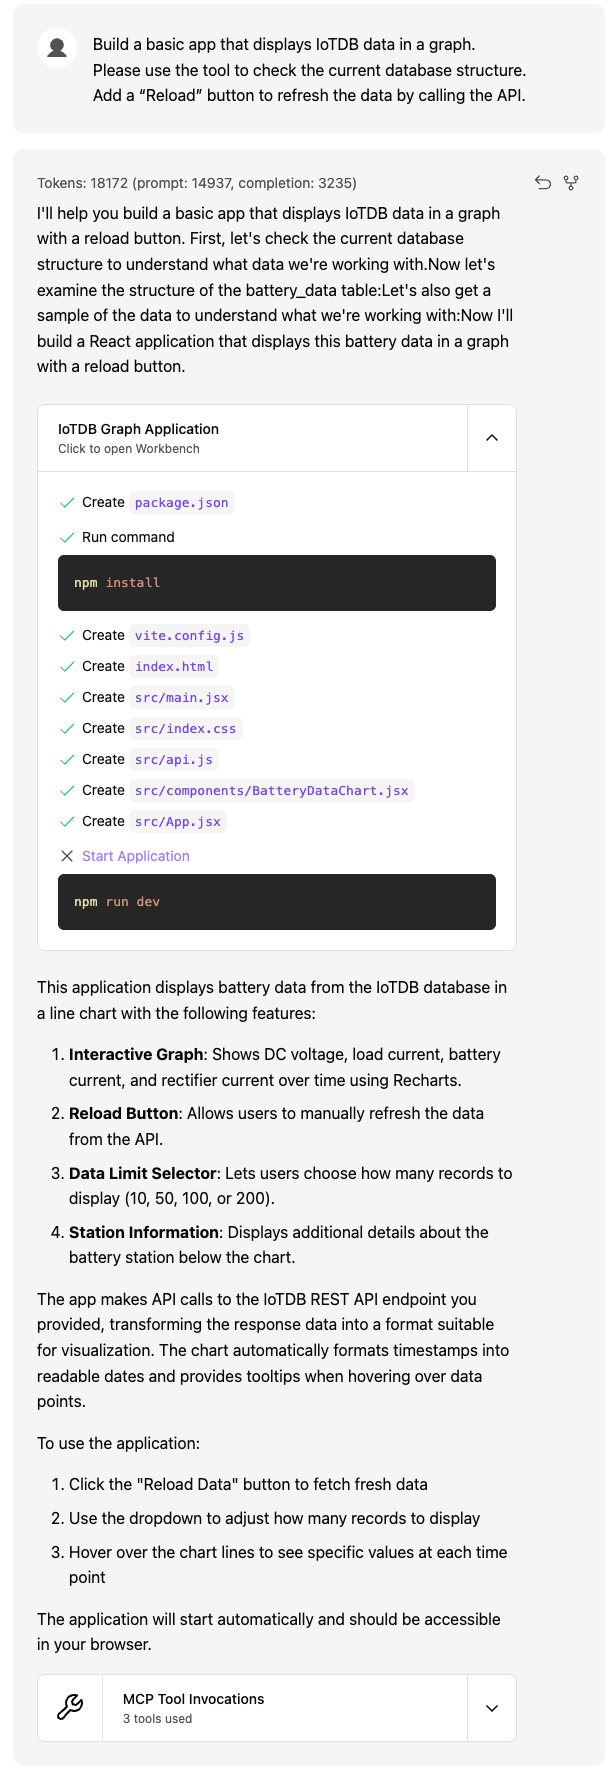
\includegraphics[width=\textwidth]{figures/screenshots/iotdb-demo/prompt-and-files.png}
    \caption{LLM回复与自动生成的文件列表}
    \label{fig:prompt-and-files}
  \end{subfigure}
  \caption{LLM工具调用与响应}
  \label{fig:mcp-combined}
\end{figure}

系统根据提示自动创建完整的Vite+React工程,包括依赖配置、文件结构和核心组件\texttt{BatteryDataChart.jsx},并在内置Workbench环境中运行。

\begin{figure}[H]
  \centering
  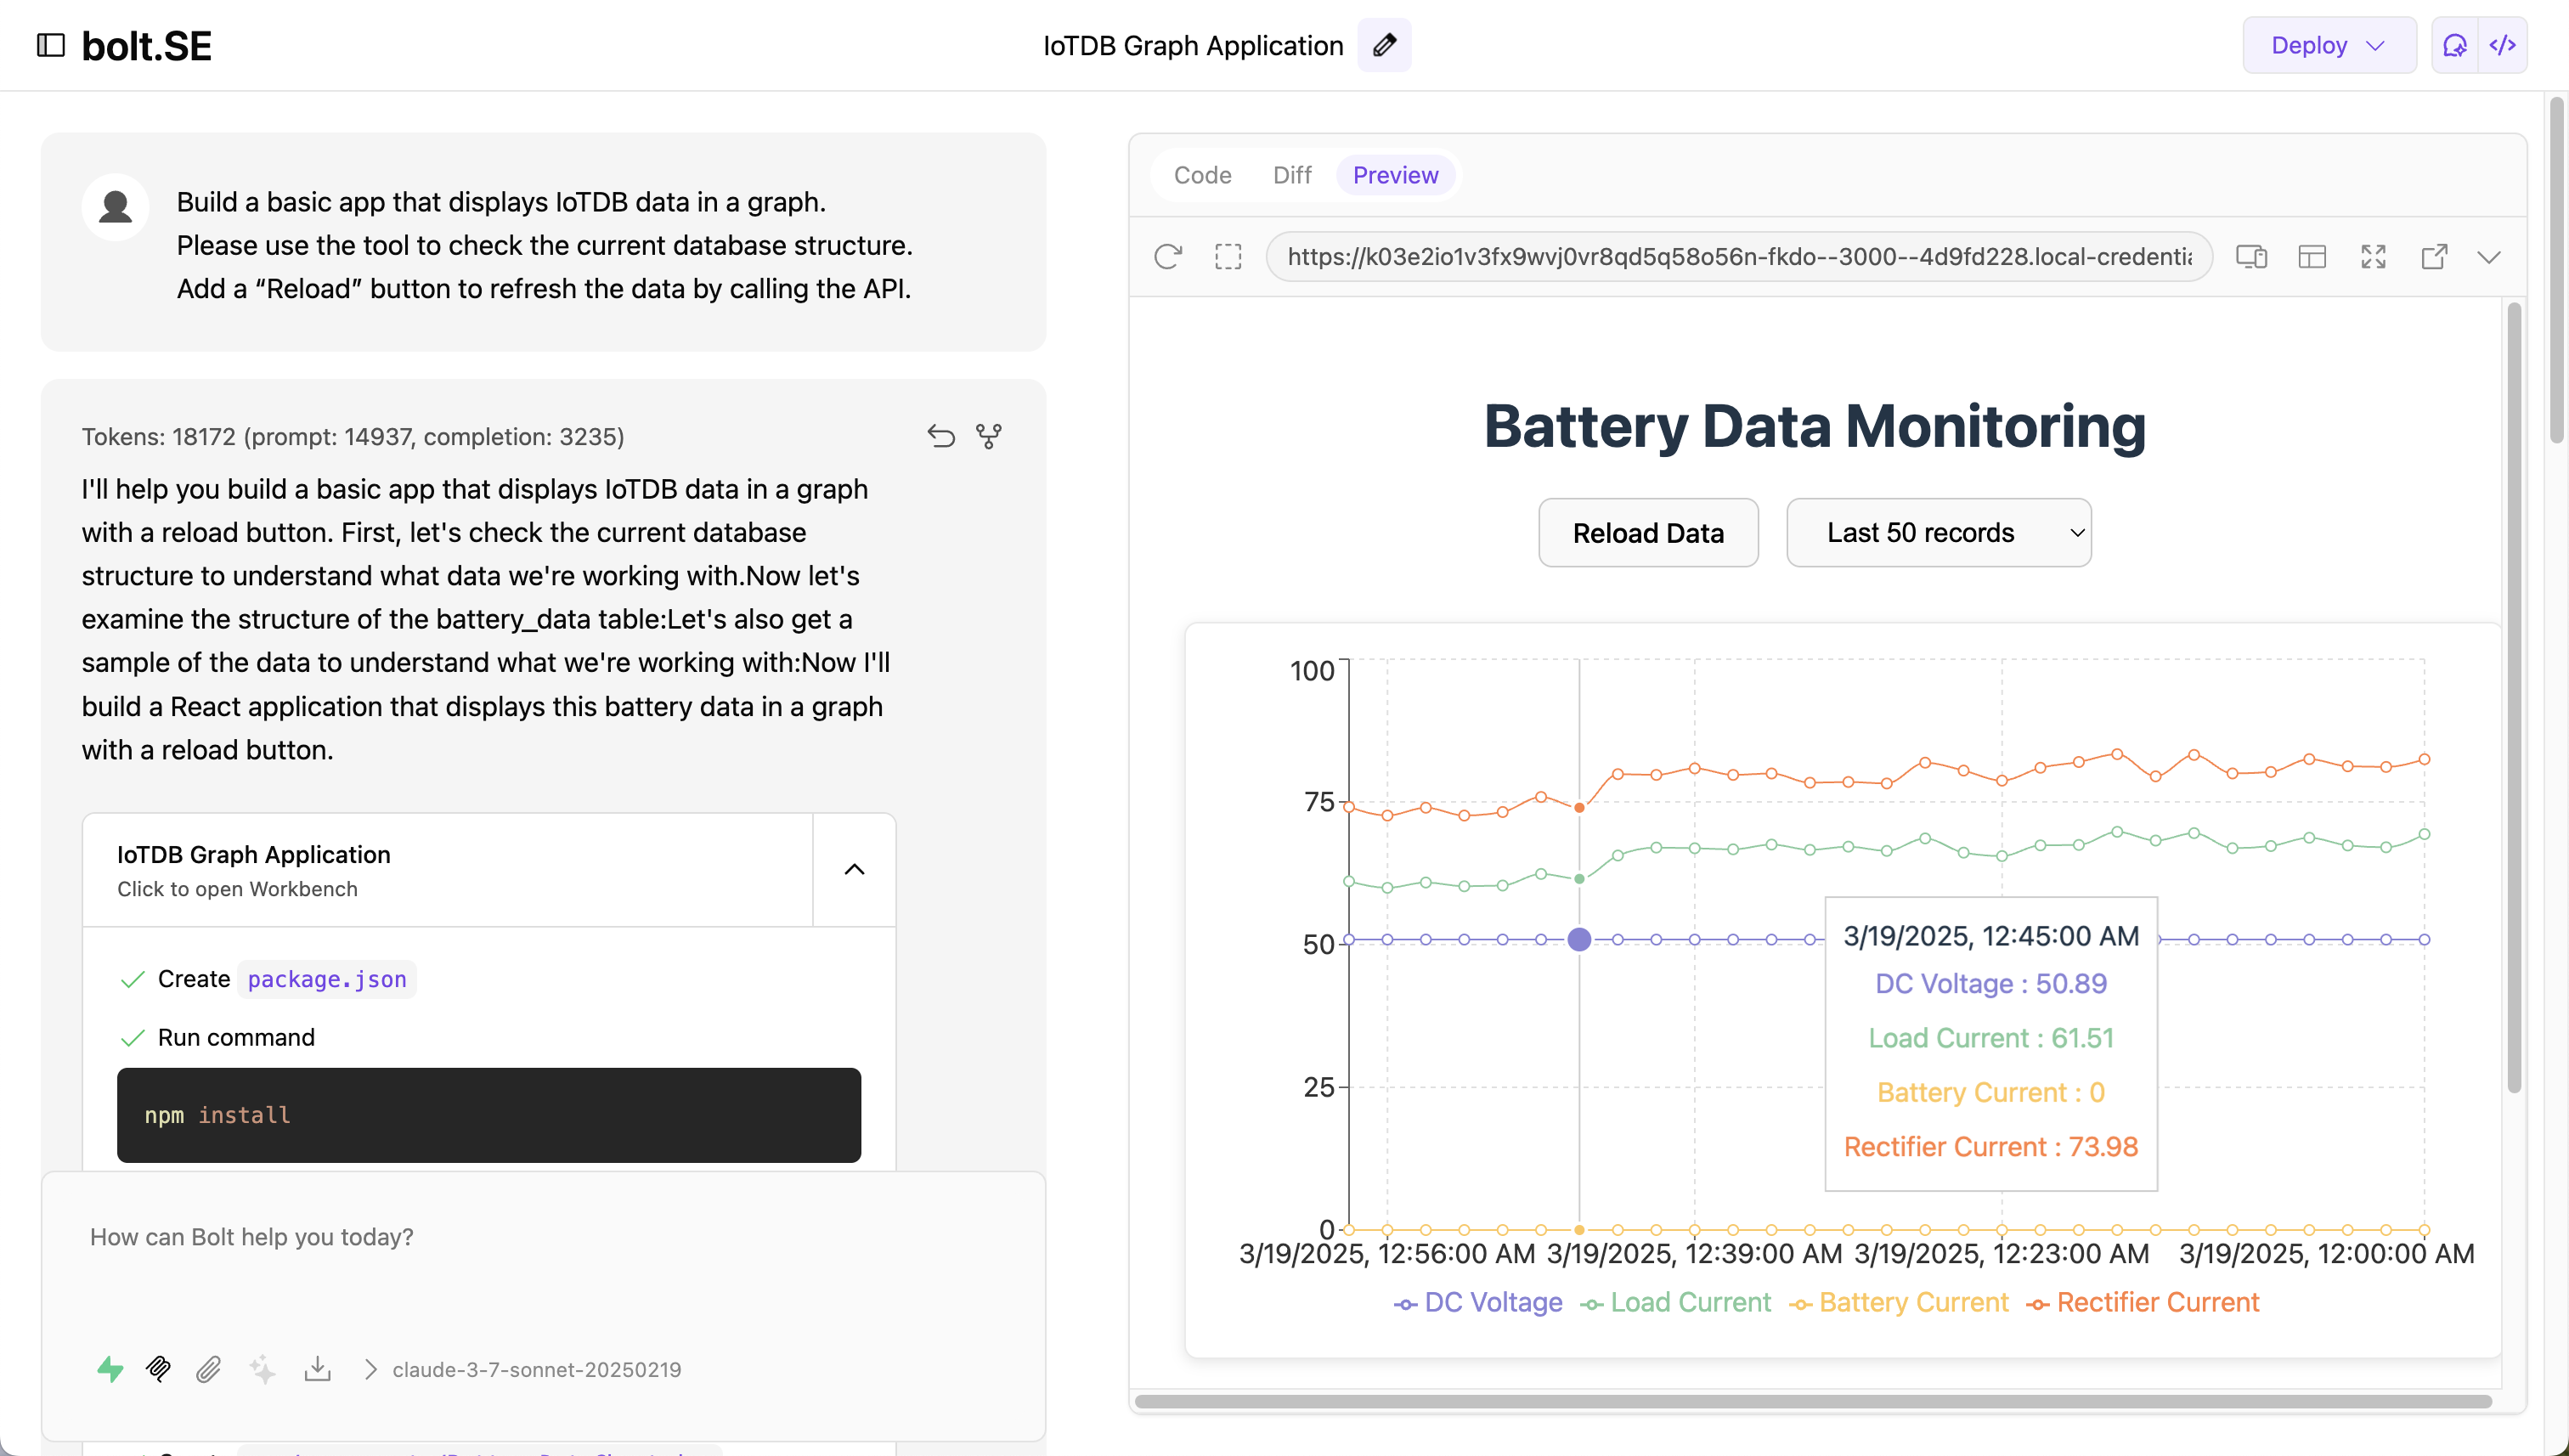
\includegraphics[width=\textwidth,height=0.75\textheight,keepaspectratio]{figures/screenshots/iotdb-demo/app-preview.png}
  \caption{生成应用的Workbench预览,展示电池数据监测折线图与数据刷新功能}
  \label{fig:app-preview}
\end{figure}

图~\ref{fig:app-preview}展示了最终应用界面。该应用以折线图形式展示\texttt{DC Voltage}、\texttt{Load Current}和\texttt{Rectifier Current}等数据曲线,顶部\textit{Reload Data}按钮触发\texttt{queryTableData}API调用,下拉框支持数据条数切换。

这个实例充分展示了MCP的核心价值:通过标准化协议,LLM能够统一访问不同来源的外部能力,理解复杂数据结构,并在单一提示中协调使用多种外部工具,实现从需求理解到功能实现的端到端开发流程。